\documentclass[a4paper,14pt]{extarticle}

\usepackage[utf8x]{inputenc}
\usepackage[T1]{fontenc}
\usepackage[russian]{babel}
\usepackage{hyperref}
\usepackage{indentfirst}
\usepackage{here}
\usepackage{array}
\usepackage{graphicx}
\usepackage{grffile}
\usepackage{caption}
\usepackage{subcaption}
\usepackage{chngcntr}
\usepackage{amsmath}
\usepackage{amssymb}
\usepackage[left=2cm,right=2cm,top=2cm,bottom=2cm,bindingoffset=0cm]{geometry}
\usepackage{multicol}
\usepackage{multirow}
\usepackage{titlesec}
\usepackage{listings}
\usepackage{listingsutf8}
\usepackage{color}
\usepackage{enumitem}
\usepackage{cmap}
\usepackage{titlesec}

\definecolor{green}{rgb}{0,0.6,0}
\definecolor{gray}{rgb}{0.5,0.5,0.5}
\definecolor{purple}{rgb}{0.58,0,0.82}

\lstdefinelanguage{none}{}

\lstset{
	language={C++},
	inputpath={../},
	backgroundcolor=\color{white},
	commentstyle=\color{green},
	keywordstyle=\color{blue},
	numberstyle=\color{gray}\scriptsize\ttfamily,
	stringstyle=\color{purple},
	basicstyle=\lst@ifdisplaystyle\footnotesize\fi\ttfamily,
	breakatwhitespace=false,
	breaklines=true,
	captionpos=b,
	keepspaces=true,
	numbers=left,
	numbersep=5pt,
	showspaces=false,
	showstringspaces=false,
	showtabs=false,
	tabsize=4,
	frame=single,
	morekeywords={NULL, DWORD, WINAPI, HANDLE, STARTUPINFO, BYTE, LPSTR, SOCKET, WSADATA, TCHAR, LPCTSTR, LPOVERLAPPED, WSABUF, SECURITY_ATTRIBUTES, SECURITY_DESCRIPTOR, TRUE, FALSE, PROCESS_INFORMATION, PIPE_UNLIMITED_INSTANCES, LPVOID, sockaddr_in},
	deletekeywords={error},
	alsoletter={_},
	sensitive=true,
	extendedchars=false,
	columns=fullflexible,
	inputencoding=utf8/cp1251,
	literate=%
		{~}{{\raise.25ex\hbox{$\mathtt{\sim}$}}}{1}%
		{-}{-}{1}
}

\makeatletter
\def\lst@outputspace{{\ }}
\makeatother

\renewcommand{\le}{\ensuremath{\leqslant}}
\renewcommand{\leq}{\ensuremath{\leqslant}}
\renewcommand{\ge}{\ensuremath{\geqslant}}
\renewcommand{\geq}{\ensuremath{\geqslant}}
\renewcommand{\epsilon}{\ensuremath{\varepsilon}}
\renewcommand{\phi}{\ensuremath{\varphi}}
\renewcommand{\thefigure}{\arabic{figure}}
\newcommand{\code}[1]{\lstinline|#1|}
\newcommand{\caret}{\^{}}
\newcommand{\ctrl}[1]{\^{}{#1}}
\newcommand{\listingwithoutput}[1]{
	\lstinputlisting[caption=\code{#1.cpp}]{src/#1/#1.cpp}
	Выполним программу \code{#1.exe}:
	\lstinputlisting[language=none]{logs/#1/#1.txt}
}

\titleformat*{\section}{\large\bfseries}
\titleformat*{\subsection}{\normalsize\bfseries}
\titleformat*{\subsubsection}{\normalsize\bfseries}
\titleformat*{\paragraph}{\normalsize\bfseries}
\titleformat*{\subparagraph}{\normalsize\bfseries}

\titlespacing{\section}{0em}{0.8em}{0.8em}

\counterwithin{figure}{section}
\counterwithin{equation}{section}
\counterwithin{table}{section}
\newcommand{\sign}[1][5cm]{\makebox[#1]{\hrulefill}}
\newcommand{\equipollence}{\quad\Leftrightarrow\quad}
\newcommand{\no}[1]{\overline{#1}}
\graphicspath{{../pics/}}
\captionsetup{justification=centering,margin=1cm}
\def\arraystretch{1.3}
\setlength\parindent{5ex}
\titlelabel{\thetitle.\quad}

\setitemize{topsep=0em, itemsep=0em}
\setenumerate{topsep=0em, itemsep=0em}

\begin{document}

\begin{titlepage}
\begin{center}
	Санкт-Петербургский Политехнический Университет Петра Великого\\[0.3cm]
	Институт компьютерных наук и технологий \\[0.3cm]
	Кафедра компьютерных систем и программных технологий\\[4cm]
	
	\textbf{ОТЧЕТ}\\ 
	\textbf{по лабораторной работе}\\[0.5cm]
	\textbf{<<Процессы и потоки в Windows>>}\\[0.1cm]
	Операционные системы\\[3.0cm]
\end{center}

\begin{flushright}
	\begin{minipage}{0.5\textwidth}
		\textbf{Работу выполнил студент}\\[3mm]
		группа 43501/3 \hfill Дьячков В.В.\\[5mm]
		\textbf{Работу принял преподаватель}\\[5mm]
		\sign[2cm] \hfill к.т.н., доц. Душутина Е.В. \\[5mm]
	\end{minipage}
\end{flushright}

\vfill

\begin{center}
	Санкт-Петербург\\[0.3cm]
	\the\year
\end{center}
\end{titlepage}

\addtocounter{page}{1}

\tableofcontents
\newpage

\section{Цели работы}

Изучение управления процессами и потоками в Windows.

\section{Программа работы}

\renewcommand{\labelenumii}{\theenumii}
\renewcommand{\theenumii}{\theenumi.\arabic{enumii}.}

\textbf{Порождение и запуск процессов}

\begin{enumerate}
	\item Неименованные каналы (pipe):
		\begin{enumerate}
			\item Создать клиент-серверное приложение, позволяющее набираемые символы в терминальном окне командной строки (сервер) отображать их в окно процесса-потомка (клиент).
			\item Создать эхо-сервер, взаимодействующий с клиентом посредством pipe.
		\end{enumerate}
	\item Именованные каналы (named pipe):
		\begin{enumerate}
			\item Реализовать между одним клиентом и сервером обмен данными, вводимыми с консоли на стороне клиента и возвращаемыми сервером обратно до получения команды exit.
			\item Реализовать между сервером и множеством клиентов обмен данными, вводимыми с консоли на стороне клиента и возвращаемыми сервером обратно до получения команды exit.
			\item Модифицировать приложение из предыдущего примера для сетевого обмена информацией.
		\end{enumerate}
	\item Сокеты (socket):
		\begin{enumerate}
			\item Реализовать программ локального и сетевую обмена с помощью сокетов с использованием потокового протокола с установлением соединения (TCP в стеке TCP/IP).
			\item Модифицировать программу для локального обмена с множеством клиентов и с доступом к общему ресурсу. Провести эксперимент с множеством клиентов при сетевом обмене, представить результаты для виртуальной и реальной сетей.
			\item Проанализировать пример применения сокетов (сетевой обмен «мгновенными» сообщениями).
			\item Привести примеры использования портов завершения. Привести пример приложения с большим количеством клиентов до 1000 (когда порты завершения оправданы), общее количество потоков не более 10.
			\item Реализовать обмен на основе UDP.
		\end{enumerate}
	\item Сигналы (signal):
		\begin{enumerate}
			\item Задать обработчик сигналов завершения для консольного приложения.
			\item Самостоятельно предложить собственную реализацию обработчика сигнала.
		\end{enumerate}
	\item Разделяемая память (file mapping):
		\begin{enumerate}
			\item Создать программу, в которой первый процесс генерирует случайное число и записывает его в буфер, доступный второму процессу, откуда он его и считывает с последующим выводом.
		\end{enumerate}
	\item Почтовые слоты (MailSlot):
		\begin{enumerate}
			\item Предложить собственную реализацию приложения, иллюстрирующую обмен информацией почтовыми слотами. Продемонстрировать возможность локального и удаленного доступа. Выполнить широковещательную передачу данных.
		\end{enumerate}
\end{enumerate}

\section{Используемая операционная система}

\begin{itemize}
	\item ОС: Windows 10 Pro
	\item Версия ОС: 1803 (сборка 17134.345)
	\item Процессоры: Intel® Core™ i7-4800MQ CPU @ 2.70GHz × 8
\end{itemize}

\newpage

\section{Создание процессов}

\subsection{Создание процесса для запуска приложения}

\paragraph{Задание.} Программа после запуска должна создать новый процесс, с помощью функции \code{CreateProcess}. В новом процессе необходимо запустить любое приложение (например, \code{notepad.exe} или \code{calc.exe}). Для контроля можно вывести идентификаторы созданного процесса и потока, а затем завершить основную программу.

\listingwithoutput{task1}

После запуска программы в новом окне был запущен блокнот \code{notepad.exe}. Информация о созданном процессе была возвращена через указатель на структуру \code{processInfo}.

\subsection{Создание процессов при работе с конфигурационным файлом}

\paragraph{Задание.} Программа, получает имя конфигурационного файла из командной строки, открывает конфигурационный файл, читает строки и создает для запуска каждой команды отдельный процесс.

\listingwithoutput{task2}

\begin{figure}[H]
	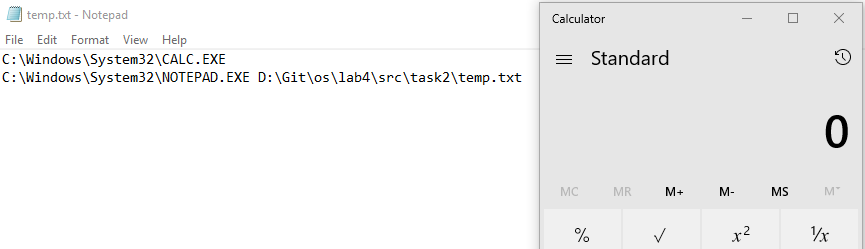
\includegraphics[width=\linewidth]{task2.png}
	\caption{Результаты выполнения \code{task2.exe}}
\end{figure}

Из результатов видно, что в новых процессах были запущены калькулятор (\code{calc.exe}) и блокнот (\code{notepad.exe}) с конфигурационным файлом.

\paragraph{Задание.} Доработаем программу. Пусть программа получает имя конфигурационного файла из командной строки, открывает его с помощью \code{fopen()}, читает построчно функцией \code{fgets()}. После прочтения каждой строки, если она не пуста, создается процесс, в командную строку которого пишется прочитанная строка. Если создать процесс не удалось, программа пробует читать конфигурационный файл дальше.

\listingwithoutput{task3}

Сначала программа была запущена без параметров, что привело к выводу ошибки. После этого имя конфигурационного файла было передано как аргумент программы. Аналогично предыдущей программе, в новых процессах были запущены калькулятор (\code{calc.exe}) и блокнот (\code{notepad.exe}) с конфигурационным файлом. Пустая строка во входном файле была корректно обработана.

\newpage

\section{Создание и управление потоками}

\subsection{Создание нескольких потоков}

\paragraph{Задание.} Программа должна создавать два потока, выводящих в бесконечном цикле <<1>> и <<2>> соответственно. После создания дополнительных потоков, поток-родитель завершается: если программа запущена без параметров, то вызывается \code{system("pause")} и \code{return 0}, иначе вызывается \code{ExitThread(0)}.

\listingwithoutput{task4}

Из результатов видно, что в первом случае произошло завершение всего процесса после нажатия клавиши, а во втором -- завершился только главный поток (программа была завершена с помощью нажатия \ctrl{C}).

\subsection{Разработка программы, в которой время жизни процесса и порождаемых в нем потоков задается как параметр}

\paragraph{Задание.} Программа должна получать 2 параметра -- количество создаваемых потоков и время жизни всего приложения. С интервалом в 1 сек каждый рабочий поток выводит о себе информацию и отслеживает состояние переменной, которая устанавливается в заданное значение по истечении времени жизни процесса.

\listingwithoutput{task5}

В программе было создано 3 потока, каждый из которых отслеживал состояние переменной \code{runFlag}. После установки \code{runFlag} в \code{false}, порожденные потоки завершились.

\section{Управления приоритетами процессов и потоков}

\subsection{Управление классом приоритета потока}

\paragraph{Задание.} Подготовить программу, в которой у каждого из потоков свой приоритет отличный от других. Все они выполняют одинаковую работу, например, увеличивают каждый свой счетчик. Накопленное значение счетчика, таким образом, отражает относительное суммарное время выполнения потока.

Кроме того, для более точного определения распределения времени между потоками, необходимо производить вычисления используя одно ядро процессора. Для этого напишем функцию \code{useSingleCore()}, внутри которой вызывается функция \code{SetProcessAffinityMask()} с маской ядер, которые процесс может использовать для выполнения.

\listingwithoutput{task6}

Из результатов видно, что значения приоритетов потоков были распределены от -15 (\code{THREAD\_PRIORITY\_IDLE}) до 15 \code{THREAD\_PRIORITY\_TIME\_CRITICAL}. Программа была запущена с аргументом 2, что соответствует установке таймера на 2 секунды. Из значений счетчиков видно, что потоки с приоритетами \code{THREAD\_PRIORITY\_HIGHEST} и \code{THREAD\_PRIORITY\_TIME\_CRITICAL} получили процессорного времени значительно больше других. Кроме того, по неизвестной причине поток с наименьшим приоритетом (\code{THREAD\_PRIORITY\_IDLE}) получил процессорного времени больше, чем оставшиеся 4 потока с более высокими приоритетами.

\subsection{Управление классом приоритета процесса}

\paragraph{Задание.} Усложним задачу и дополним ее возможностью управлять классом приоритетов процесса.

\listingwithoutput{task7}

Из результатов видно, что ни один из потоков не поменял динамический приоритет в процессе выполнения. Больше всего процессорного времени получили поток с приоритетом \code{THREAD\_PRIORITY\_HIGHEST} и поток с приоритетом \code{THREAD\_PRIORITY\_TIME\_CRITICAL}. Потоки с низким приоритетом почти не получили процессорного времени, т.е. наблюдается <<ресурсное голодание>>.

\subsection{Анализ поведения системных функций динамического управления приоритетами процессов и потоков}

\paragraph{Задание.} С помощью программы определить, назначается ли динамическое изменение приоритетов по умолчанию, на все ли потоки воздействует функция \code{SetProcessPriorityBoost}, возможно ли разрешение отдельному потоку в процессе динамически изменять приоритет, если для процесса это запрещено.

\listingwithoutput{task8}

Из результатов видно, что по умолчанию для процессов и потоков разрешено динамическое изменение приоритетов. Затем для второго потока было запрещено изменение динамического приоритета с помощью вызова функции \code{SetThreadPriorityBoost}. Если запретить динамическое изменение приоритетов для процесса (\code{SetProcessPriorityBoost}), то изменение также будет запрещено и для всех потоков. Тем не менее, возможно разрешить отдельному потоку в процессе динамически изменять приоритет, несмотря на то, что для процесса это запрещено.

\newpage

\section{Задания для самостоятельного выполнения}

\subsection{Исследование работы программ в зависимости от приоритета базового потока}

\paragraph{Задание.} Исследуйте результаты работы программы \code{task7} в зависимости от того, какой приоритет назначается базовому потоку: \code{IDLE}, \code{BELOW\_NORMAL}, \code{NORMAL}, \code{ABODE\_NORMAL}, \code{HIGH}, \code{REALTIME}.

Выполним \code{task7} со всеми возможными приоритетами процесса.
\lstinputlisting[language=none]{logs/task7/all.txt}

Видно, что установить процессу приоритет \code{REALTIME\_PRIORITY\_CLASS} не удалось, а процессу был назначен приоритет \code{HIGHEST}. Приведем сводную таблицу значений счетчиков в зависимости от приоритета процесса и потока:

\begin{table}[H]
	\centering
	\def\tabcolsep{5pt}
	\caption{Зависимость значений счетчиков от приоритета процесса и потока}
	\begin{tabular}{|c|c|c|c|c|c|c|}
		\hline
		Thread/Process & \code{IDLE} & \code{BELOW} & \code{NORMAL} & \code{ABOVE} & \code{HIGH} & \code{REALTIME} \\ \hline
		\code{IDLE} & 3 & 3 & 3 & 2 & 2 & -- \\ \hline
		\code{LOWEST} & 3 & 3 & 3 & 2 & 2 & -- \\ \hline
		\code{BELOW} & 3 & 3 & 3 & 2 & 2 & -- \\ \hline
		\code{NORMAL} & 3 & 3 & 4 & 2 & 2 & -- \\ \hline
		\code{ABOVE} & 1230279 & 1310870 & 4 & 1390225 & 1467519 & -- \\ \hline
		\code{HIGHEST} & 2602627 & 2622270 & 3892063 & 2619412 & 2631990 & -- \\ \hline		\code{TIME\_CRIT} & 1372349 & 1311213 & 3892553 & 1229249 & 1164385 & -- \\ \hline
	\end{tabular}
\end{table}

\subsection{Таблица относительных приоритетов}

\paragraph{Задание.} Модифицируйте программу \code{task7} для заполнения таблицы приоритетов текущими данными вашего эксперимента. Сделайте выводы.

Для этого перед выводом итоговых значений счетчиков нормализуем их таким образом, чтобы значение максимального счетчика было равно 15. Выполним программу \code{task9} с установкой различных приоритетов процессу. 
\lstinputlisting[language=none]{logs/task9/task9.txt}

Видно, что как и в предыдущем пункте установить процессу приоритет \code{REALTIME\_PRIORITY\_CLASS} не удалось. Приведем сводную таблицу относительных значений приоритетов потоков в зависимости от приоритета процесса.

\begin{table}[H]
	\centering
	\def\tabcolsep{10pt}
	\caption{Относительные значения приоритетов потоков в зависимости от приоритета процесса}
	\begin{tabular}{|c|c|c|c|c|c|c|}
		\hline
		Thread/Process & \code{IDLE} & \code{BELOW} & \code{NORMAL} & \code{ABOVE} & \code{HIGH} & \code{REALTIME} \\ \hline
		\code{IDLE} & 1 & 1 & 1 & 1 & 1 & -- \\ \hline
		\code{LOWEST} & 1 & 1 & 1 & 1 & 1 & -- \\ \hline
		\code{BELOW} & 1 & 1 & 1 & 1 & 1 & -- \\ \hline
		\code{NORMAL} & 1 & 1 & 1 & 1 & 1 & -- \\ \hline
		\code{ABOVE} & 8 & 9 & 1 & 7 & 9 & -- \\ \hline
		\code{HIGHEST} & 15 & 15 & 15 & 15 & 15 & -- \\ \hline
		\code{TIME\_CRIT} & 8 & 7 & 15 & 9 & 7 & -- \\ \hline
	\end{tabular}
\end{table}

Из результатов видно, что таблица довольно сильно отличается от теоретической, а поток с приоритетом \code{HIGHEST} получал процессорного времени больше других независимо от приоритета процесса.

\subsection{Мониторинг и фиксация динамического изменения приоритетов}

\paragraph{Задание.} С помощью утилит CPU Stress, позволяющих нагружать систему, и утилиты мониторинга \code{Process Explorer} (или иных утилит) зафиксируйте динамическое изменение приоритетов, приведите результаты в отчете.

Вместо использования утилит CPU Stress, запустим программу \code{task7} с установкой приоритета процесса в \code{HIGHEST}. С помощью утилиты \code{Process Explorer} откроем окно \code{Properties} процесса с вкладкой \code{Threads}.  

\begin{figure}[H]
	\centering
	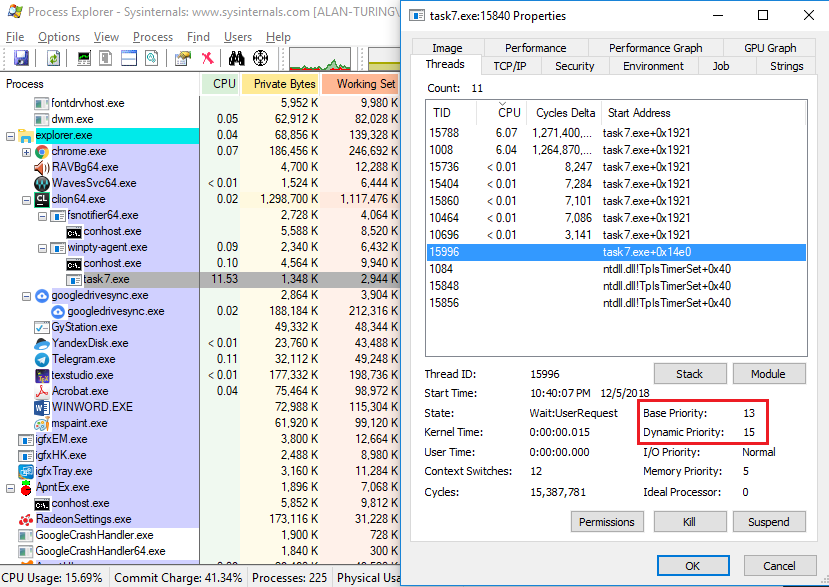
\includegraphics[width=0.9\linewidth]{dynamic.png}
	\caption{Динамическое изменение приоритета}
\end{figure}

Видно, что приоритет одного из запущенных потоков был повышен на два пункта -- с 13 до 15.

\subsection{Наследование дескрипторов}

\paragraph{Задание.} Создайте программу, демонстрирующую возможность наследования:

\begin{enumerate}
	\item дескриптора порождающего процесса,
	\item дескрипторов открытых файлов,
\end{enumerate}
для выполнения этого задания следует учесть, что по умолчанию наследование в Windows отключено и для возможности наследования, необходимо:

\begin{itemize}
	\item разрешить процессу-потомку наследовать дескрипторы,
	\item сделать дескрипторы наследуемыми.
\end{itemize}

Для того, чтобы сделать дескриптор файла наследуемым, необходимо внутри программы \code{parent.exe} передать функции \code{CreateFile()} структуру \code{SECURITY\_ATTRIBUTES} с установленным флагом \code{bInheritHandle}. Для того, чтобы разрешить потомку наследовать дескрипторы, передадим пятым параметром функции \code{CreateProcess()} значение \code{TRUE}. Сам дескриптор при этом передается через аргументы командной строки \code{char *argv[]} программы \code{son.exe}.

\lstinputlisting[caption=\code{parent.cpp}]{src/parent_son/parent/parent.cpp}
\lstinputlisting[caption=\code{son.cpp}]{src/parent_son/son/son.cpp}

Запустим программу \code{parent.exe}:
\lstinputlisting[language=none]{logs/parent_son/parent_son.txt}

Видно, что родительский процесс создал дескриптор файла, после чего вызывал функцию \code{CreateProcess}. После этого начал выполнятся порожденный процесс, в котором еще раз вывелся полученный дескриптор. После выполнения содержимое файла \code{file.txt} оказалось следующим:
\lstinputlisting[language=none]{logs/parent_son/file.txt}

Таким образом, с помощью вызова \code{CreateFile()} и \code{CreateProcess()} со специальными флагами возможно наследование файловых дескрипторов.

\section{Выводы}

В процессе выполнения данной работы:

\begin{itemize}
	\item рассмотрены функции создания процессов и управления потоками;
	\item изучены приоритеты процессов и потоков, а также функции для их изменения;
	\item рассмотрено наследование дескрипторов.
\end{itemize}

\section*{Список использованных источников}

\begin{enumerate}
	\item Душутина Е.В. - Системное программное обеспечение. Практические вопросы разработки системных приложений [Текст] -- 2016.
	\item Таненбаум Э. - Современные операционные системы [Текст] -- 2015.
	\item Handle Inheritance / Microsoft Docs [Электронный ресурс]:\\
		{\small\url{https://docs.microsoft.com/en-us/windows/desktop/sysinfo/handle-inheritance}} 
\end{enumerate}

\end{document}
